\section{Laboratory work implementation}

\subsection{Tasks and Points}

\begin{itemize}
 \item Setarea interfeței vizuale;
 \item Crearea metodelor pentru prelucrarea evenimentelor și atașarea lor la GUI;
 \item Crearea codului \textit{Core};
 \item crearea metodelor pentru efectuarea operațiilor matematice.
\end{itemize}

\subsection{Analiza lucrarii de laborator}

\par Link la repozitoriu: \url{https://insert.your.link.here} 

\par Am efectuat lucrarea pe platforma .NET\cite{net}, folosind drept mediu de dezvoltare Microsot Visual Studio\cite{vs} și C\# în calitate de limbaj de programare. Proiectul este alcătuit din două module: GUI și Core, care conține metodele pentru efectuarea calculelor și sunt folosite în modulul GUI.

\par Pentru crearea modulului grafic am utilizat un proiect de tip WinForms unde am adăugat pe o formă butoanele necesare și un label în care va fi afișat textul introdus.

\begin{figure}[ht]
 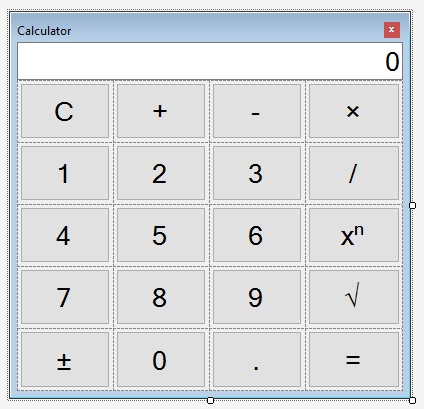
\includegraphics[scale=1]{imagini/interfata}
 \centering
 \captionof{figure}{Interfața aplicației}
\end{figure}

\par După aceasta am creat metode pentru fiecare eveniment necesar și le-am legat cu acțiunile butoanelor. Pe lângă evenimentele de click au fost prelucrate și cele de KeyPress. Am întâlnit o problemă cu evenimentul apelat la tastarea butonului "Enter", se executa evenimentul imlicit din windows, care simulează click pe butonul activ la moment, în loc de metoda definită. Aceasta a fost soluționată prin supraâncărcarea metodei \textbf{ProcessCmdKey}.

\begin{figure}[ht]
 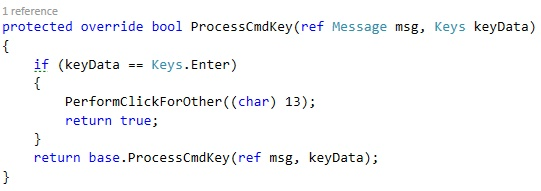
\includegraphics[scale=1]{imagini/override}
 \centering
 \captionof{figure}{Supraâncărcarea metodei ProcessCmdKey}
\end{figure}

\subsection{Imagini}

\begin{figure}[ht]
 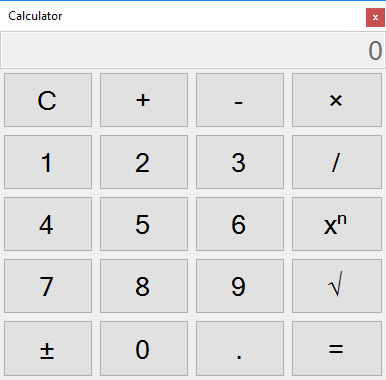
\includegraphics[scale=1]{imagini/1-initial}
 \centering
 \captionof{figure}{Fereastra inițială}
\end{figure}

\begin{figure}[ht]
 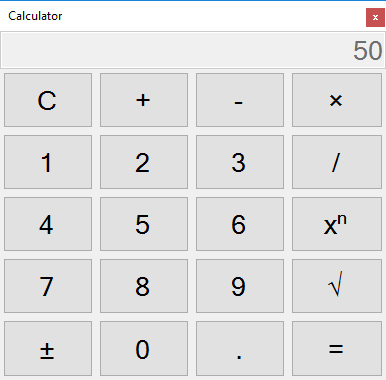
\includegraphics[scale=1]{imagini/2-write}
 \centering
 \captionof{figure}{Introducerea datelor}
\end{figure}

\begin{figure}[ht]
 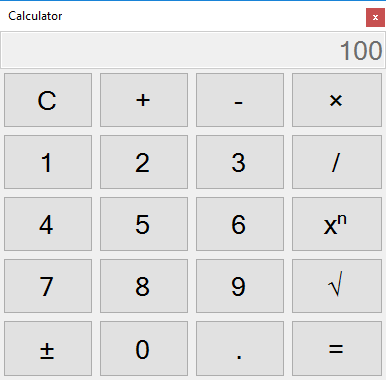
\includegraphics[scale=1]{imagini/3-50+50}
 \centering
 \captionof{figure}{Rezultatul expresiei 50+50}
\end{figure}

\begin{figure}[ht]
 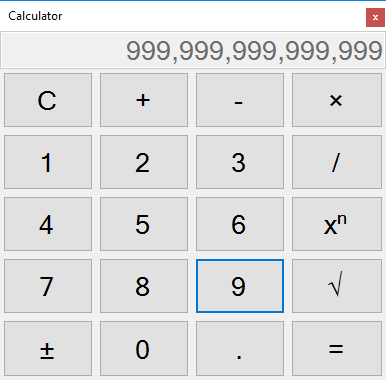
\includegraphics[scale=1]{imagini/4-max}
 \centering
 \captionof{figure}{Numărul maxim}
\end{figure}

\begin{figure}[ht]
 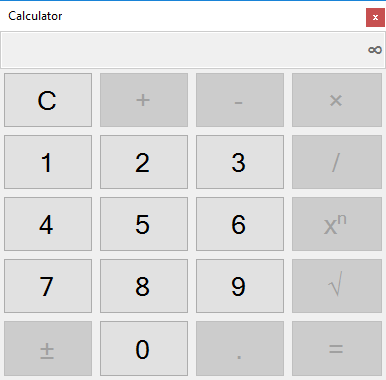
\includegraphics[scale=1]{imagini/5-overflow}
 \centering
 \captionof{figure}{Caz de overflow}
\end{figure}

\begin{figure}[ht]
 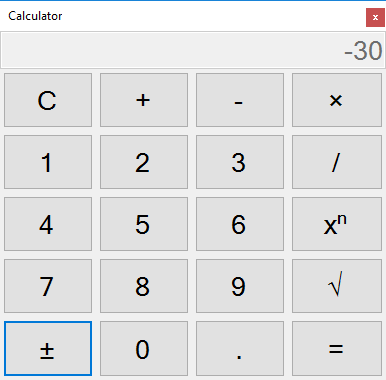
\includegraphics[scale=1]{imagini/6-sign-change}
 \centering
 \captionof{figure}{Operația de schimbaer a semnului}
\end{figure}

\begin{figure}[ht]
 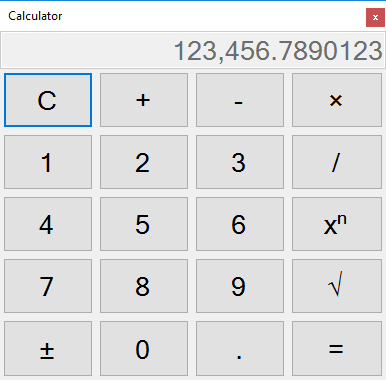
\includegraphics[scale=1]{imagini/7-decimal}
 \centering
 \captionof{figure}{Introducerea unui număr zecimal}
\end{figure}

\clearpage